% Chapter 2
\setstretch{1}
\chapter{Artist-Led Technical Collaboration}\thispagestyle{empty} % Main chapter title

\label{Chapter2} % For referencing the chapter elsewhere, use \ref{Chapter1} 

\lhead{Chapter 2. \emph{Artist-Led Technical Collaboration}} % This is for the header on each page - perhaps a shortened title
\setstretch{2}

\section{Design Research: Artist Collaboration}
screenPerfect began with an artistic collaboration, where as a programmer, I worked closely with an artist to reproduce the technical elements of a working practice in order to make it available to other artists in a similar field. This specificity allowed us to develop a very simple tool that solves a minimal set of problems in a tidy fashion, while expanding the repeatable part of a single artist's process - the idea of how linked videos \textit{should} connect together on multiple screens - to a tool that can be used by other artists. Arts-led research promotes a point of view distinct from the typical business-forward viewpoint, preferring to ask "how might we" than to say "this is how we will." As a developer, it can be difficult to tie work to a given set of problems, or to ensure it has value to an audience outside oneself. Therefore, collaboration gives access to a set of problems that may seem easy but are frequently technically complex and challenging - and therefore rewarding. 

\section{Software Development Methods: Agile}
The agile method of software development is based on the Agile Manifesto, much as the underlying feminist elements of this project are based on the Cyborg Manifesto and Cixous' manifesto for \textit{\'{e}criture f\'{e}minine}. Agile is a response to previous software design practices, called "Waterfall," where software frameworks are laid out and heavily documented in advance of production. Waterfall methods are popular in major software companies, which rely on extensive documentation to communicate between business units. Waterfall emphasizes planning over software production or delivery deadlines.

The idea of agile was described in 2001 by a group of software developers \parencite{agile}. By using an agile practice of responsive, user-centered design, screenPerfect's interaction model was designed through a series of discussions with key stakeholders, followed by iterative code revisions to a rough first prototype. This can be seen as a hacker-oriented means of development, reflecting Sadie Plant's statement in Zeros and Ones that reverse engineering - "starting at the end, and then engaging in a process that simultaneously dismantles the route back to the start" \parencite{plant}. Agile specifically emphasizes individuals and interactions over processes and tools, working software over comprehensive documentation, customer collaboration over contract negotiation, and responding to change over following a plan \parencite{agile}. 

The screenPerfect development process emerged from a series of linked videos on YouTube, as laid out by Hannah Epstein. We then reviewed strengths and weaknesses of this model: the ability for a large audience with public interlinked video files but the downside of long load times and ads on pages detracting from the video content. In addition, this required uploading films at low quality to a remote server. From the initial prototype, we asked how the process could be improved, particularly for an exhibition context. 

The game processes laid out in Youtube were converted to a "how might we" - a series of static files presented as interactions in still film. Hannah Epstein laid out an idea of how the video screens should work together. I confirmed that this system was theoretically possible using websockets - a communication protocol - loaded into a Node.JS application. From there, I wrote a Node app that served basic video files to multiple browser screens simultaneously. This started as a chat application, serving text to three screens simultaneously over websockets. We then replaced the text with video files, layered a control structure over the videos using plaintext JSON files to replace a reliance on a database structure.

A database was not originally required for \textit{psXXYborg}, the original game built by Hannah Epstein using screenPerfect, or later games using that exlusive engine, because installing a database is an additional step that nontechnical end users cannot be relied upon to find straightforward. Every step of the development process was intended to result in code that is legible to anyone who can read javascript, while being absolutely straightforward to use for a nontechnical video author. 

In development conversations, it became clear that YouTube, in addition to having many distracting advertisements, was very slow to load. This is a problem with reliance on external networks: they cannot be as fast as locally served files. Epstein specifically emphasized speed, smooth loading, and video based in static rather than streaming or live files. These needed to be served within a closed environment to an attentive audience. 

Scripting languages are especially good at this type of development work. I reached out to other developers and asked how they would solve this problem. They came back to me with a variety of answers - some used PHP, some used Python, all of them relied on JS for their front end. In researching different ways to solve the basic problem - passing a variable back and forth through wireless technology to select two on-screen videos at almost the same time - I discovered the Node.JS software framework, a software package designed to permit developers to use Javascript on both the server and client side of a web application. From here, I designed a client-server-control model - Figure 3.1, the screenPerfect Software Communication Model. This relied on an interlinked system of hardware and software designed to respond to what resources it found available in its load space. 

Epstein relied on the h.264 format for her video production, which necessitated an early reliance on the Safari web browser, as HTML5 video does not yet have a settled public codec at the time of writing. Due to conflicts relating to codec patenting, one of many such conflicts that underly the "free" internet, Safari supports H.264 where Chrome supports webm via the V8 engine, the same engine that supports the Node framework. Webm is a compact video format, which results in smaller file sizes and lower bandwidth costs, which eventually affects both load time and playback lag on client machines. 

Figure 2.1 describes the ultimate screenPerfect program code flow, which relies on an always-open two way communication channel based on the relatively novel websockets communication protocol. Essentially, on software boot, a given browser loads a client window and a control window, which open a channel to the server and a passthrough to one another. When something changes, the other channel - always open - displays that change to all paired clients. What is being changed in this case is what game data is dynamically loaded to a single screen at any given time. The flow chart describes how that software's communications patterns travel on a user interaction with a given touchpoint.

\clearpage
\begin{figure}[h!]
 \centering
 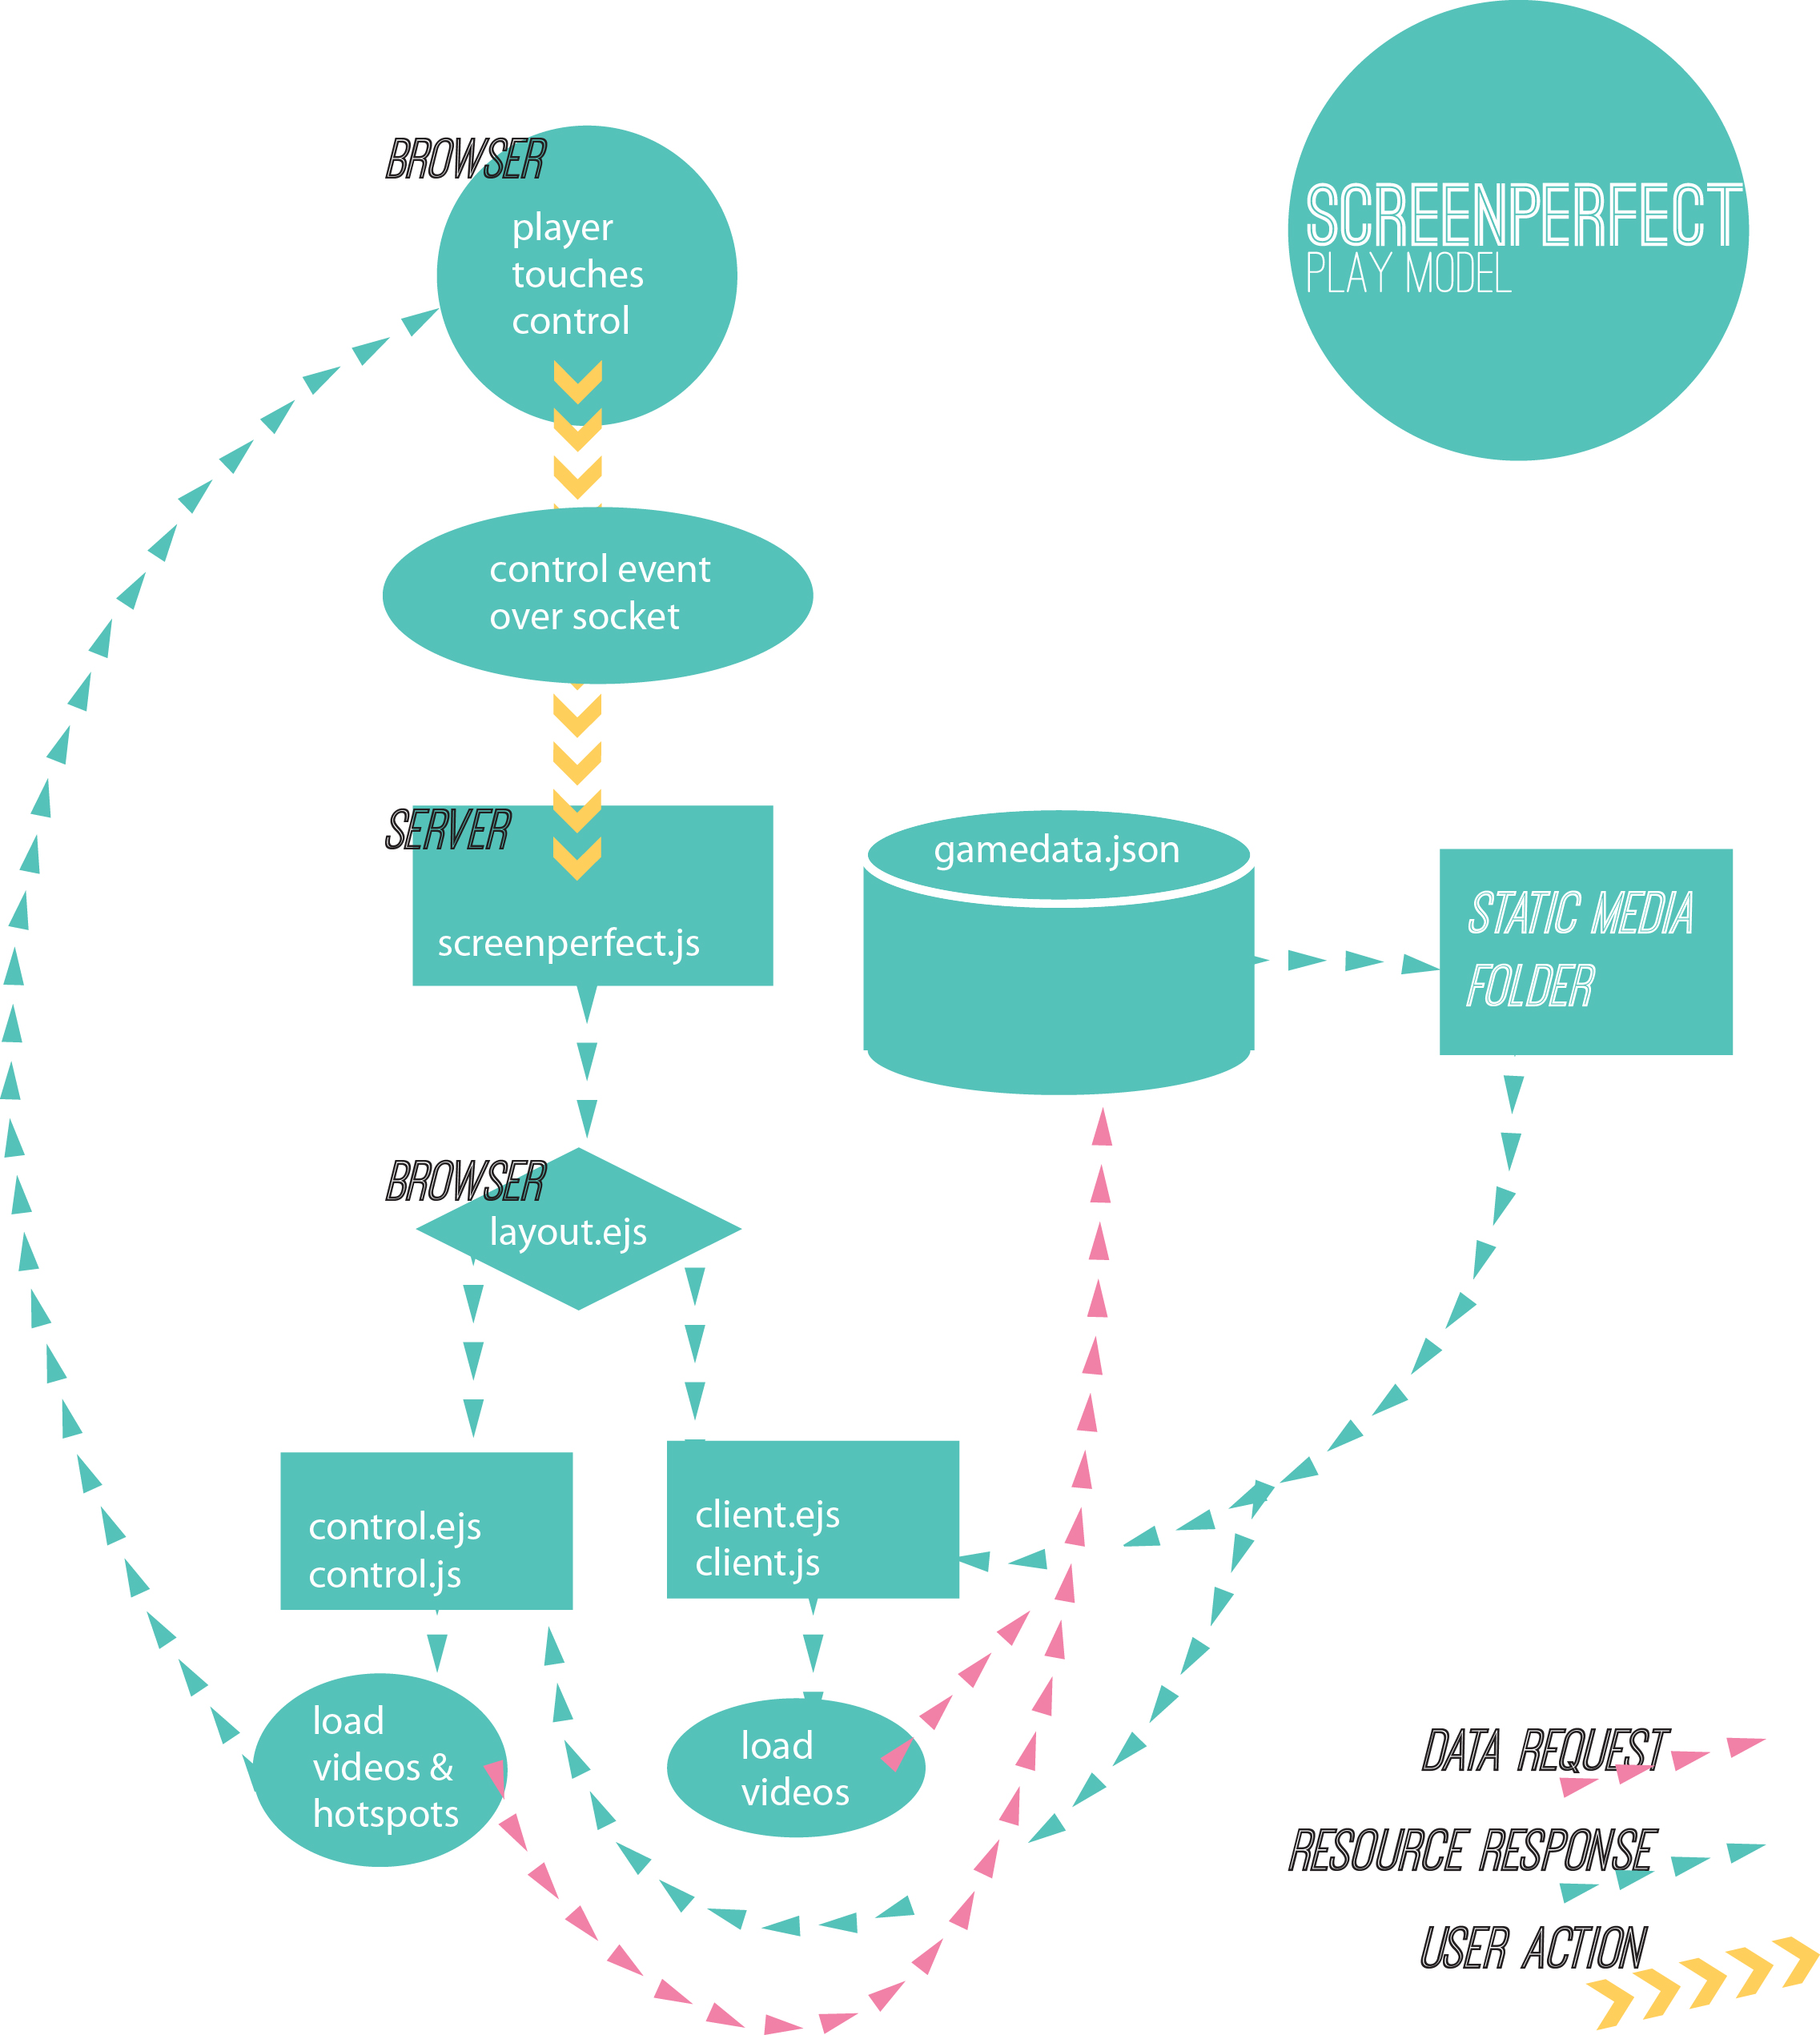
\includegraphics[width=\textwidth]{spCodeFlow}
 \caption{screenPerfect software communication model}
\end{figure}
\clearpage

\subsection{Full Motion Video Games and Mobile Interactive Screens}
FMV (Full Motion Video) games are an old format, relatively speaking. FMV began almost as soon as chapter selection became available on the laser disc systems of the 1980s, with 1983's game \textit{Dragon's Lair} by Rick Dyer and Don Bluth, the first entry in what would become a strange sub-genre. FMV was successful through 1984 but quickly failed due to the expense of laser disc systems and the relative cost of game development and play. The 1985 Halcyon system cost \$2000 - adjusted for inflation, \$4,347.88 in 2014 - and offered only two games. The most well-known FMVs outside of \textit{Dragon's Lair} are \textit\textit, released in 1992, and \textit{Phantasmagoria}, from 1996. \textit{Night Trap} went on to become part of the congressional hearings of offensive video game material along with \textit{Mortal Kombat}, the first widely popular fighting game to allow people to rip out one another's spines. \textit{Phantasmagoria} was better known as the first adult-oriented game released by Roberta Williams, famed for her involvement in Sierra's \textit{King's Quest} point-and-click adventure game series \parencite{encyclopediavideogame}.

FMV and branched narrative games differ from cartridge-based action games in that they do not typically feature the same immediate feedback of a score going up and the instant player controls of a more typical 2D or 3D action game. Instead, players select what will happen next at key intervals. Older games are easy to display, so long as working hardware can be found, because they rely on consistent materiel for installation. Digital interactive forms, particularly those on the internet, live in a more malleable format. They can change, or be taken down, at any time. The gameplay experience of a console game can be had even when disconnected from the internet – in fact, the Nintendo 3DS, a pocket console, outsold every other system on the market in 2013. It is speculated that its success is due largely to the fact that the 3DS is a portable system that does not connect to the broader internet unsupervised \parencite{3dssales}. This reliability is something that is rare to find in more complex computers: sometimes, as argued by Don Norman in "The Design of Everyday Things" \parencite{norman}, it is best to have a single thing do one thing really well. 

FMV games remain interesting enough to engage fans. This is partly due to the well-documented nostalgic appeal of certain forms of entertainment, digital games in particular sparking sites such as videogamenostalgia.com and hashtags on Tumblr like \#videogamenostalgia or \url{http://fuckyeahchrono.tumblr.com/}. FMV have been recreated using Youtube and preserved from laser discs and DVDs \parencite{laserdiscarcade}. Phantasmagoria can easily be found in complete playthrough on Youtube, where the annotation system makes recreating a point-and-click environment trivial (\url{https://www.youtube.com/watch?v=oAXC-MwfpHA}). Nonetheless, they were heavily systems-dependent and are tricky to develop, given the difficulties surrounding copyrighted video works and public distribution - how to transmit something that contains so many different pieces of video information?

Another example of portable electronic interaction is the smartphone. Initially this technology seems not so great for bringing people together in the same space, as the privacy of the phone has been seen as undermining or distracting. It is possible to see this instead as a source of potential: people examine things one-on-one with their devices and then will share them with their peers.

Smartphones are inherently private systems - a category of hardware referred to as a "personal device" - used in public places. Personal devices have all kinds of content on them, from games to e-mail to tax returns. Apps, paid for and downloaded, are understood to be private even when their terms of licence imply that they are the sole property of the developer. Websites are public places one can "visit" on a phone, an external resource supplied to a personal locale. This leads to a set of assumptions on behalf of interaction developers: an application is a private thing, paid for, and downloaded to a private space within the phone, whereas a web page is a public resource that can be viewed in private on a phone. A smartphone is also a single encapsulated controller, with all necessary inputs provided by its touch surface. For interactive artwork, this means that some assumptions can be made.

The first is that the audience of an interactive art piece is likely to be familiar with how to interact with a touchscreen but also may be distracted. It cannot be assumed that they will download or pay for an application sight unseen for the sake of art, because that would constitute an expenditure of resources without reference but they can be asked to go to a web page. People commonly use their phones in public. Therefore it seems reasonable to ask them for the minimal engagement of looking at something specific, this time art served only within the gallery. 

There are already games that aim to subvert this separation. Systems have been built to take advantage of the power of pocket computers. A notable effort is "Spaceteam," \parencite{spaceteam} a ‘Simon-Says' game for teams of up to four players. The application pairs to itself across phones by using a common network connection, having players in the same physical space cooperate to pilot a star ship. This allows players to make use of a device with which they are already comfortable to cooperate and share an experience.

This shared experience makes it possible to privately host a public space. A private host is a computer that is unreliably connected to the broader internet - perhaps occasionally, perhaps not at all - which serves an application using technologies that make it appear to be part of that internet to people who access the resource using their phone. These are web applications, served in private, to a public but small gallery space, to preserve the context of the application while relying on the user's own resources in the form of a phone to give the work a personal context within the public-private site. In this way, a private site which cannot connect to the broader internet can take advantage of the design model of internet communication to serve works without them being decontextualised to anyone who wishes to navigate to them more broadly.

In this way, web art is no longer the broad exploration of net.art but becomes instead a preservable, repeatable installation.

screenPerfect, a web application served locally, takes advantage of an assumed set of smartphone users in galleries having access to the internet in their pockets. The internet is both bigger and smaller than the wider network – the internet that includes Google and other multi-national internet corporations. Rather than relying on the external resources of remote servers, screenPerfect provides a private wifi point and what is called a "captive portal" to let players pair with one another and the server, control a large screen, and interact with a piece of video art in a localized area. This means that an artist can control the exhibition space for their work, design the experience of the work, and ensure that their audience will experience the work in a specific context. It also ensures that technicians can access the underlying engine should something go wrong during the installation.

\section{Game Engines}
A game engine is a collection of software designed to make it possible for a team of artists, developers, musicians, and producers to work together to produce a complete digital experience. Traditionally, game engines are used to produce 2D or 3D experiences using assets such as 2D sprites or 3D player character/interaction models, backgrounds, interaction assets - crates, for example - music, and scripts in a programming language to tie all of these together into gameplay. 

Some popular professional engines at the time of writing are Unity3D, which features native mobile integration and ease of scripting in both Javascript and C\#; Crytek, which comes with many high-end 3D resources preloaded for high definition graphic support; the Unreal Engine, which is quite stable and useful to experienced teams that prefer more control over their work.

There are popular hobby engines that de-emphasize programming as well, such as GameMaker, which is prized for PC compatibility, Game Salad for OSX, and Construct 2, which is PC-only but has a powerful engine to manage game physics and interactions. These engines all assume a certain type of player interaction: they are designed to enable designers to produce specific types of games, such as a "shooter" or a "platformer," similar in style to the \textit{Call of Duty} franchise or Nintendo's \textit{Mario} series. The interactions available are easily understood as a language of action by their players, provided players have previous experience with digital gameplay.

\subsection{Twine}
Twine is a game engine that allows designers to build HTML5 text narratives that branch into a choose-your-own-adventure game. screenPerfect was inspired in no small part by the popularity of both Twine and video on the internet. Twine encourages expressive type styling and elements of multimedia, including music, and game screens but does not require these elements for a complete interactive narrative. Twine did not yet support video narratives in 2013.

The Twine engine was popularized by DIY gaming celebrity Anna Anthropy in her 2012 book \textit{Rise of the Videogame Zinesters} \parencite{anthropy}. Anthropy's book calls for a dramatic DIY practice to articulate personal experience in video games. She strongly promotes Twine as an easy way to begin the effort of designing personal games. Since then, hundreds of Twines - the adopted term for narratives built in Twine - have seen release.

\subsection{Multiscreen Video Technology}
Dual screen technology, or more accurately, multi-screen synchronous web technology, is one of the big new ideas being heavily backed by Google in 2013. As a consequence, its Chrome browser has been designed to support software developed with a specific suite of frameworks, many of which are wholly supported by Google. 
This being said, Google supports Node and Chrome both, so multi-screen technology using web browsers is open to people for no more investment than a new programming language. screenPerfect relies on Node.JS, which is based on Google's V8 engine.

The architecture of screenPerfect is wholly new but the concept is based on the Dataton Watchout system, which encourages producers to develop large multi-screen single video experiences on custom hardware. Dataton Watchout costs approximately \$40,000 dollars per installation, which makes an inexpensive alternative appealing from a creative standpoint. screenPerfect permits people to use existing hardware to synch multiple videos to one set of controls. This is also distinct from another related tool, ChromeCast, that allows people to wirelessly pair a television with a touchscreen for control and consumption of the touchscreen at a larger size. ChromeCast requires an ecosystem of development that is presented as inclusive chiefly to those already invested in the startup scene. Therefore, these tools have been built from a position of inclusivity. By releasing them through a group of largely non-technical artists, I have chosen to pursue a research path that deprivileges the role of the technology compared to the role of the artist within a given system.

\subsection{Licensing}
One of the ways these problems are dealt with is through licensing. The Creative Commons at creativecommons.org expresses their mission as follows: "Creative Commons develops, supports, and stewards legal and technical infrastructure that maximizes digital creativity, sharing, and innovation." It is therefore an appropriate open standard licence for creative practice. A preferred licence for software development is the MIT Licence, which is closer to the Gnu Public Licence but does not preclude making money from one's open source work. 

\subsection{Science Fiction Inputs}
My own idea for how this project would work is derived from Cory Doctorow's \textit{Pirate Cinema}, which features a scene wherein characters climb trees then use projectors already built into their phones, assemble a movie theatre from nothing more than sheets and ropes in the trees \parencite{doctorow}. I feel this sort of mesh-networked sharing is much more likely than a continued reliance on the surveilled internet for sharing copyrighted and copyrighted- material derived works. Since I could not find a system that would permit this type of sharing on the internet, I felt that this project would provide a good opportunity to build one.

\section{Code as Context-Sensitive Writing}
As a creative project, code is a tricky thing to pin down. It must say something structurally, yet it reveals the internal architecture of its authors. Programming leaves loose ends. An excellent piece of software is likely to require input from a wide array of specialists in graphic design, interface development, and logic. There is an inevitable tendency to produce flaws - bugs - that cause the program to fail. Once complete, it is likely that finished software will fall out of fashion. Just as there is no way to call a piece of writing finished, because another word can always be added or cut loose, code is subject to scope creep. 

Code lives, like writing, in context and within an ecosystem. Code answers to its context. As Alexander Galloway says in his book "Gaming: Essays On Algorithmic Culture," without the machines that run it, code is without consequence \cite{galloway}. Within those machines, code may have a concrete effect on the world around it. For that reason it continues to be valued. To code is to attempt to write a way of addressing the world, a single way that must take into consideration all the assumptions of people who tried to address the world before, and, with future-proofing, the world after. 

\section{Software Design}
A software interface is the part of the software that a person interacts with directly where a software engine is the part of the code that detects and defines what a computer can do with that interaction. 
The interface of software is just as important as the engine, however, because a poorly designed interface will confuse a user thereby rendering the experience of using the engine potentially opaque. 
screenPerfect's roots are as a software engine, which takes user action and then does things with it. The user interacts with the interface that speaks to the engine which then returns values to whichever interface the user has selected.

\subsection{screenPerfect Engine|Interface Layout}
In the case of screenPerfect, the interface is laid out in three parts. The first part is the setup screen, the second is the control screen, and the third is the generic client screen. The setup area is by far the most complex area. It is used by game designers to load their media to the database and lay out the links between those files. This is the essence of a game made in screenPerfect: which choice will a player make to navigate the system as designed by the artist?

The further screens are the client and control screens. screenPerfect supports up to ten client screens and ten control screens, although the interface only exposes a polyphony of client windows, while restricting artists to a single control set for simplicity's sake.

The layout of screenPerfect's editing tools did not work very well for authors who were not already part of the prototyping process. Therefore, as part of the extension of the software for NoJam, Bento Box-Miso reauthored the editing interface of the software. 
The final editing layout is clean, though less expressive than the original design. Rather than hidden tabs, everything is displayed on launch. This permits authors to see their video files during the entire game editing process, which greatly speeds game creation. 
What follows are screencaptures of the pre-fork game jam variant of screenPerfect.

\newpage
\begin{figure}[h]
 \caption{screenPerfect NoJam editor, Asset Population tab.}
 \centering
 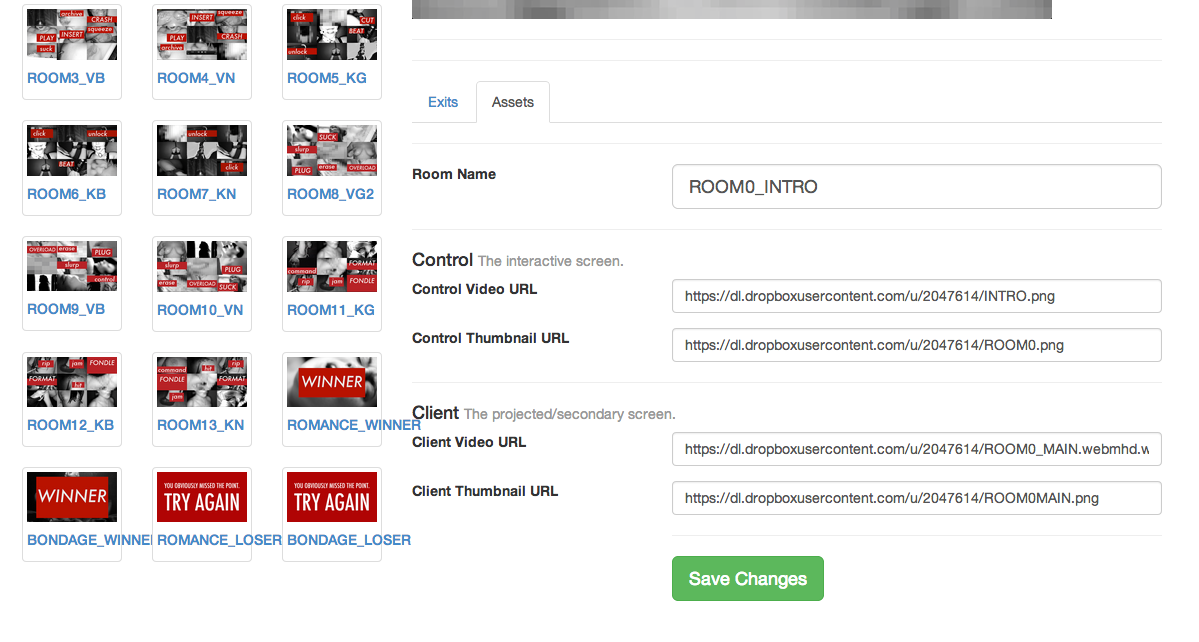
\includegraphics[width=\textwidth]{editSoftAssetTab}
\end{figure}

\begin{figure}[h]
 \caption{screenPerfect NoJam editor, Exit Population tab.}
 \centering
 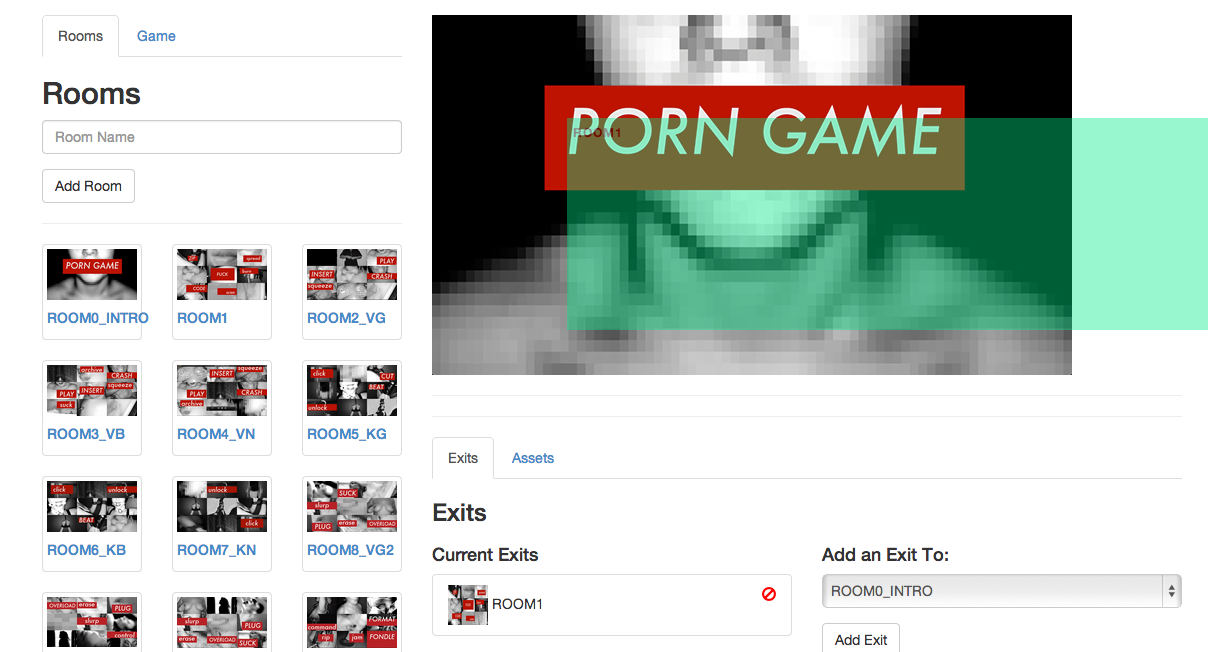
\includegraphics[width=\textwidth]{editSoftExitTab}
\end{figure}

\newpage 